\subsection{התלות של השגיאה ברדיוס $R$}
\begin{figure}[h!]
    \centering
    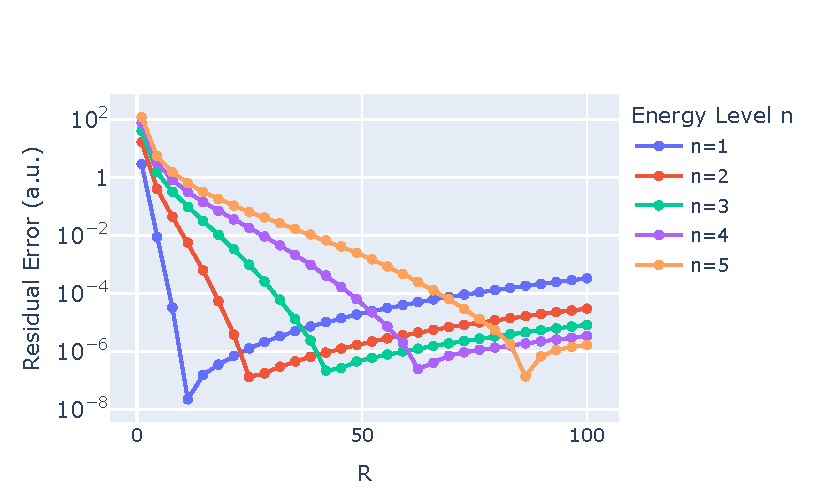
\includegraphics[width=0.7\linewidth, trim=0 0 0 2cm, clip]{plots/r_dependence/residual_error.eps}
    \caption{השגיאה עבור ערכים משתנים של $R$. ניתן לראות כי לכל רמת אנרגיה יש איזה רדיוס אופטימלי.}
    \label{fig:r_dependent_error}
\end{figure}

ניתן לראות ב\autoref{fig:r_dependent_error} כי עבור כל אחד מרמות האנרגיה קיים איזה רדיוס $R=a_n$ אופטימלי בו השגיאה מינימלית. ניתן להבין את התופעה הזאת מהסתכלות על פונקציית הגל של כל אחת מהרמות. ניתן לראות שרוב במידע מתרכז בתוך רדיוס מסויים, שגדל עם רמות האנרגיה. כאשר בוחרים $R<a_n$  מאבדים חלק מהמידע, ואני משער שעבור $R\ll a_n$ כאשר נגדיל את $K$ נקבל שיפור פחות משמעותי מאשר אם נבחר $R\approx a_n$. מצד שני, כאשר בוחרים $R>a_n$ אנחנו מתחילים להוסיף נקודות באזורים שכמעת ולא מכילים מידע, כך שעבור $K$ קבוע נקבל פחות נקודות באזור שמכיל מידע.